\subsection{Linear Systems}
\subsubsection{Linear Combinations}
A combination of vectors $s_1\vec{a}_1$ and $s_2\vec{a}_2$, $s_1,\,s_2\in\R$ is called a \textit{linear combination} of $\brcurly{\vec{a}_1,\,\vec{a}_2}$\\
The set of all linear combinations of a set is called the \textit{span} of the set of vectors.\\
Ex: $\spann\brcurly{\brangle{1,0,0},\,\brangle{0,1,0},\,\brangle{0,0,1}}=\R^3$\\
Ex2: $\spann\brcurly{\brangle{1,0,0},\,\brangle{0,1,0}}=\R^2$\\
Ex3: If $\vec{a}=\brangle{2,3}$ and $\vec{b}=\brangle{1,2}$, is $(1,1)$ in the span of $\brcurly{\vec{a},\,\vec{b}}$? If so, find the linear combination.
\begin{align*}
    &\text{Require $s$ and $t$ such that }s\vec{a}+t\vec{b}=\brangle{1,1}\\
    &s\brangle{2,3}+t\brangle{1,2}=\brangle{1,1}\\
    &\brangle{2s+t,\,3s+2t}=\brangle{1,1}\\
    &\eqnsystem{2s+t=1\\3s+2t=1}\Ra s=1,\,t=-1\\
    &\to\text{ any point, }(c_1,c_2)\text{ can be written as a linear combination of }\vec{a}\text{ and }\vec{b}\\
    &\therefore\spann\brcurly{\vec{a},\,\vec{b}}=\R^2
\end{align*}
A collection of vectors is called \textit{linearly dependent} if some nontrivial (not all 0) combination of equal zero. Otherwise, it is called \textit{linearly independent}\\
$\vec{a},\,\vec{b},\,\vec{b}$ are linearly dependent if
$$\det\matrixx{-\vec{a}-\\-\vec{b}-\\-\vec{b}-}=0$$
or if
$$\matrixx{|&|&|\\\vec{a}&\vec{b}&\vec{b}\\|&|&|}\matrixx{|\\\vec{0}\\|}$$
has rank $<n$. i.e. no unique solution\\
Ex: Is $\brangle{1,0,1},\,\brangle{1,1,0},\,\brangle{0,1,1}$ linearly independent?
\begin{align*}
    &\det\matrixx{1&0&1\\1&1&0\\0&1&1}=\detmatrix{1&0\\1&1}-0\detmatrix{1&0\\0&1}+\detmatrix{1&1\\0&1}=1-0+1=2\neq0\\
    &\therefore\text{ linearly independent}
\end{align*}
A collection of $n$ linearly dependent vectors in $\R^n$ dimensional space is called a \textit{basis}. So if $\vec{a},\,\vec{b},\,\vec{b}$ are linearly independent they form a basis and any vector, $\vec{x}$, can be formed from a linear combination of $\vec{a},\,\vec{b},\,\vec{b}$.
$$\matrixx{|&|&|\\\vec{a}&\vec{b}&\vec{b}\\|&|&|}\matrixx{|\\\vec{k}\\|}=\matrixx{|\\\vec{x}\\|}$$


\subsubsection{Gaussian Elimination}
Say we have a system of 3 equations and 3 unknowns. We can use an augmented matrix to solve this system.
\begin{align*}
    \text{Ex: }\eqnsystem{x_2+x_3=1\\x_1+x_2=2\\x_1+x_2+x_3=3}=\augmatrix{0&1&1\\1&1&0\\1&1&1}{1\\2\\3}
\end{align*}
Once in augmented matrix form on the right, we can perform the following elementary row operations:
\begin{itemize}
    \item Multiply a row by a non-zero number
    \item Add a multiple of one row to another row
    \item Interchange two rows
\end{itemize}
Using these operations we can perform Gaussian elimination to put the matrix into echelon form and come to our solution.\\
Gaussian Elimination Method:
\begin{enumerate}
    \item kill off first column so that there is only one nonzero number remaining
    \item Use a row with a 0 first entry to kill off the second column
    \item Continue the process until you are able to solve for a variable
    \item Use the variable you solved for to work backwards and solve for the rest
\end{enumerate}
\begin{align*}
    \text{Ex: }&\augmatrix{0&1&1\\1&1&0\\1&1&1}{1\\2\\3}\to\augmatrix{1&1&0\\0&1&1\\1&1&1}{2\\1\\3}\to\augmatrix{1&1&0\\0&1&1\\0&0&1}{2\\1\\1}\\
    &x_3=1\\
    &x_2=1-x_3=1-1=0\\
    &x_1=2-x_2=2\\
    &\vec{x}=\brangle{2,0,1}
\end{align*}
\subsubsection{Solution Spaces}
Not all systems will have a unique solution. Some may have no solutions and some may have infinite solutions
\begin{align*}
    \text{Ex2: }\augmatrix{1&1&0\\0&1&1\\0&0&0}{1\\0\\1}
\end{align*}
if you look at the last row, it states that $0=1$. This implies that there is no solution to the system
\begin{align*}
    \text{Ex3: }&\augmatrix{1&2&3\\1&1&1}{0\\1}\to\augmatrix{1&2&3\\0&-1&-2}{0\\1}
\end{align*}
In this example, we have no equation to determine $x_3$ so we call it a free variable and assign it a variable value $t$ instead of a number.
\begin{align*}
    &x_3=t\\
    &-x_2-2x_3=1\Ra x_2=-1-2x_3=-1-2t\\
    &x_1+2x_2+3x_3=0\Ra x_1=-2x_2-3x_3=-2(-1-2t)-3t=2+t\\
    &\vec{x}=\brangle{2+t,-1-2t,t}
\end{align*}
Notice, the solution space is also the equation of a line.\\
A handy way to imagine solution spaces is through lines and planes. In a 3x3 matrix, each row represents a plane and the solution is the intersection of the three planes. Similarly, if two rows are linearly dependent, we will effectively only have two planes and the solution space will be the intersection of these two planes which is a line.\\
One way to determine the number of solutions a system has is using rank.\\
The \textit{rank} of a matrix is the number of nonzero rows of the matrix in echelon form.\\
$r$ represents the rank of the matrix\\
$r_A$ represents the rank of the augmented matrix (inclusive of the rightmost column)\\
If we consider a matrix to be of size $m\times n$ then $m$ is the number of rows and $n$ is the number of columns. ($n$ is also the number of variables).
\begin{itemize}
    \item If $\rank(A)<\rank(\brsquare{A|b})$, there are no solutions (irrational argument)
    \item If $\rank(A)=\rank(\brsquare{A|b})=n$, there will be a unique solution
    \item If $\rank(A)=\rank(\brsquare{A|b})<n$, there will be infinite solutions
\end{itemize}
A special type of augmented matrix comes from homogeneous systems. These have 0 for all the constant terms and the matrix will either have one solution ($\vec{x}=0$) or infinite solutions.
$$\augmatrix{a_{11}&a_{12}&a_{13}\\a_{21}&a_{22}&a_{23}\\a_{31}&a_{32}&a_{33}}{0\\0\\0}$$


\subsubsection{Resistor Networks}
Mesh Current Method:
\begin{enumerate}
    \item Determine variables: the current in every loop ($I_1,\,I_2,\,\ldots I_n$) and the voltage drop across the current sources ($E_1,\,E_2\,\ldots E_n$)
    \item Set up equations so that the sum of the voltage in each loop is zero and equations that relate the specific currents of the current source
    \item Set up in a matrix and solve for the unknowns
\end{enumerate}
*The current must be travelling in the same direction in each loop (i.e. arbitrarily set all clockwise)\\
*We consider the current specific to the loop we are considering to be positive\\
Ex: If the current source is $4A$, find the voltage drop across all resistors and the current source\\
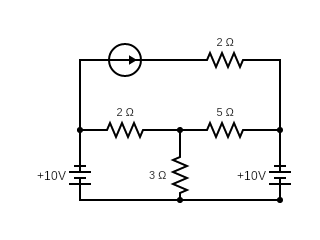
\includegraphics[scale=0.8]{LinearAlgebraPictures/ResisterNetworksEx.png}
\begin{align*}
    &\text{Loop 1: }-E=2I_1=5(I_1-I_3)+2(I_1-I_2)=0\\
    &\text{Loop 2: }10+2(I_2-I_1)+3(I_2-I_3)=0\\
    &\text{Loop 3: }5(I_3-I_1)-10+3(I_3-I_2)=0\\
    &\text{Current Source: }I_1=4\\
    &\eqnsystem{2I_2+5I_3+E=36\\5I_2-3I_3=-2\\-3I_2+8I_3=30}\\
    &\augmatrix{2&5&1\\5&-3&0\\-3&8&0}{36\\-2\\30}\leadsto\eqnsystem{I_1=4A\\I_2\approx 2.3871A\\I_3\approx 4.6452A\\E=8V}\\
    &V_{R_2}=2|I_1-I_2|\approx 3.2V\\
    &V_{R_5}=5|I_1-I_3|\approx 3.2V\\
    &V_{R_3}=3|I_2-I_3|\approx 6.8V
\end{align*}

\subsubsection{Polynomial Interpolation}
If we define $\phi_0(t)=1,\ \phi_1(t)=t,\ldots,\ \phi_d(t)=t^d$ then a polynomial of degree $d$ is of the form
$$p(t)=c_0\phi_0(t)+c_1\phi_1(t)+\cdots+c_d\phi_d(t)$$
We can say that the polynomials $\phi_k(t)$ form a basis of a $d$-degree polynomial, $\mathbb{P}_d$ and the set $\brcurly{\phi_0(t),\ldots,\phi_d(t)}$ is called the \textit{monomial basis} of $\mathbb{P}_d$.\\
We wish to find a polynomial, $p(t)=\brcurly{c_0+c_1t+\cdots+c_dt^d:\ c_0,c_1,\ldots,c_d\in\R}$, that interpolates the points $(t_0,y_0),(t_1,y_1),\ldots,(t_n,y_n)$.\\
Each data point will give an equation:
\begin{align*}
    &\eqnsystem{c_0+c_1t_0+c_2t_0^2+\cdots+c_dt_0^d=y_0\\ c_0+c_1t_1+c_2t_0^2+\cdots+c_dt_1^d=y_1\\ \vdots\\ c_0+c_1t_d+c_2t_d^2+\cdots+c_dt_d^d=y_d}
\end{align*}
which gives $d+1$ equations for $d+1$ unknowns.\\
Writing this in the form $A\vec{c}=\vec{y}$, we get
$$\matrixx{1 & t_0 & \cdots & t_0^d\\ 1 & t_1 & \cdots & t_1^d\\ \vdots & \vdots & \ddots & \vdots\\ 1 & t_d & \cdots & t_d^d}\matrixx{c_0\\ c_1\\ \vdots\\ c_d}=\matrixx{y_0\\ y_1\\\vdots\\ y_d}$$
where the matrix $A$ is called the \textit{Vandermode matrix}.\\
The Vandermode matrix has the identity that
$$\det(A)=\prod_{0\leq i<j\leq d}(t_j-t_i)$$
Ex: For a 3x3 Vandermode matrix,
\begin{align*}
    &\detmatrix{1 & t_0 & t_0^2\\ 1 & t_1 & t_1^2\\ 1 & t_2 & t_2^2}=(t_1-t_0)(t_2-t_0)(t_2-t_1)
\end{align*}
Ex: Find a polynomial that passes through the points $(-1,2),(0,1),(1,4)$
\begin{align*}
    &A=\matrixx{1 & -1 & 1\\ 1 & 0 & 0\\ 1 & 1 & 1},\ \vec{y}=\matrixx{2\\1\\4}\\
    &A\vec{c}=\vec{y}=\augmatrix{1 & -1 & 1\\ 1 & 0 & 0\\ 1 & 1 & 1}{2\\1\\4}\leadsto\augmatrix{1 & -1 & 1\\ 0 & 1 & -1\\ 0 & 0 & 2}{2\\-1\\4}\\
    &c_3=2\Ra c_2=-1+c_3=1\Ra c_1=2+c_2-c_3=1\\
    &\vec{c}=\matrixx{1\\1\\2}\Ra p(t)=1+t+2t^2
\end{align*}
A downside to polynomial interpolation is that the condition number of the Vandermode matrix gets very large with an increase in the amount of points.
\subsubsection{Cubic Spline Interpolation}
Cubic spline interpolation is the method of interpolating data points using a piecewise cubic function. The rational is that a cubic function allows you to match the function, its derivative, and its 2nd derivative, giving it the appearance of a very smooth interpolation of the data.\\
If we have $N+1$ data points, $(t_0,y_0),(t_1,y_1),\ldots,(t_N,y_N)$, it will be defined by $N$ cubic polynomials defined by the general equation
$$p_k(t)=a_k(t-t_{k-1})^3+b_k(t-t_{k-1})^2+c_k(t-t_{k-1})+d_k,\ t\in[t_{k-1},t_k]$$
This leaves us with $4N$ unknowns we have to solve for.\\
We can get our unknowns using the following constraints:
\begin{itemize}
    \item Left endpoints: $p_k(t_{k-1})=y_{k-1}$ gives $N$ equations
    \item Right endpoints: $p_k(t_k)=y_k$ gives $N$ equations
    \item Continuity of $p'(t)$: $p'_k(t_k)=p'_{k+1}(t_k)$ gives $N-1$ equations
    \item Continuity of $p''(t)$: $p''_k(t)=p_{k+1}''(t_k)$ gives $N-1$ equations
\end{itemize}
We can get our last 2 equations using arbitrary boundary conditions.\\
We define the natural cubic spline to have the property that
\begin{itemize}
    \item $p''_1(t_0)=p''_N(t_N)=0$
\end{itemize}
We express the cubic spline with its coefficient matrix:
$$C=\matrixx{a_1 & a_2 & \cdots & a_N\\ b_1 & b_2 & \cdots & b_N\\ c_1 & c_2 & \cdots & c_N\\ d_1 & d_2 & \cdots & d_N}$$
We can solve for these coefficients using a behemoth of a linear system:
$$\matrixx{A(L_1) & B & & & \\ & A(L_2) & B & & \\ & & \ddots & \ddots & \\ & & & A(L_{N-1}) & B\\ T & & & & V}\matrixx{a_1\\b_1\\c_1\\ \vdots\\ a_N\\b_N\\c_N}=\matrixx{y_1-y_0\\ 0\\0\\\vdots\\ y_N-y_{N-1}\\0\\0}$$
where $L_k=t_k-t_{k-1}$ and
\begin{align*}
    A(L)=\matrixx{L^3 & L^2 & L\\ 3L^2 & 2L & 1\\ 6L & 2 & 0}& &B=\matrixx{0 & 0 & 0\\ 0 & 0 &-1\\ 0 & -2 & 0}\\
    T=\matrixx{0 & 0 & 0\\ 0 & 2 & 0\\ 0 & 0 & 0}& &V=\matrixx{L_N^3 & L_N^2 & L_N\\ 0 & 0 & 0\\ 6L_N & 2 & 0}
\end{align*}
The last 2 rows of the augmented matrix correspond to the natural cubic spline condition and would be different for a different cubic spline model.
